\documentclass[../dissertation.tex]{subfiles}

\begin{document}

\chapter{Monte Carlo Integration, Path Tracing, and Temporal Difference Learning}
\label{chap:technical}

The goal of this section is to a give you as the reader a good understanding of  the technical concepts which our work relies on. We begin with Monte Carlo integration, as the theory behind how a Monte Carlo approximation can be used to find the true value of an integral forms the mathematical basis of the path tracing algorithm. We then give a full description of the path tracing algorithm and how it relates to the \textit{rendering equation}, as well as pseudo code which we extend upon in chapter \ref{chap:td_deep_sampling}. Finally, we provide a short introduction to Reinforcement Learning and with it, temporal difference learning. This is the foundation of how both we and NVIDIA learn the incident radiance function, but the extension of how this applies to path tracing is saved until chapter \ref{chap:td_deep_sampling}.

\section{Monte Carlo Integration and Importance Sampling}
\label{sec:monte_carlo}
The theory of importance sampling for Monte Carlo integration underpins how noise in images rendered by path tracing can be reduced when using the same number of SPP. Therefore, it is necessary to have a good understanding of Monte Carlo integration and its properties, as well as importance sampling before applying it to path tracing.

\subsection{Monte Carlo Integration}
\label{sec:monte_carlo_approx}
 Monte Carlo Integration is a technique to estimate the value of an integral, equation \ref{eq:integral} represents this integral for a one-dimensional function $f$ between two points $a,b$.

\begin{equation}
\label{eq:integral}
F = \int_a^b f(x) dx
\end{equation}

Monte Carlo integration is used to approximate an integral by uniformly sampling points ($x_i$) to evaluate the integral. These solutions to the integral are essentially averaged to find an approximation to the integral, or in other words, to find the area beneath the curve formed by the function ($f$) within the integral. More formally, basic Monte Carlo integration approximates a solution to an integral using the numerical solution in equation \ref{eq:monte_carlo}. Where $\langle F^N \rangle$ is the approximation of the value of the integral $F$, using $N$ samples and $x_i$ is a sample point \cite{morokoff1995quasi}.

\begin{equation}
\label{eq:monte_carlo}
\langle F^N \rangle = (b - a) \frac{1}{N} \sum^{N-1}_{i=0} f(x_i)
\end{equation}

\begin{equation}
\label{eq:generalized_mc}
\langle F^N \rangle = \frac{1}{N} \sum^{N-1}_{i=0} \frac{f(x_i)}{\frac{1}{(b-a)}} 
 = \frac{1}{N} \sum^{N-1}_{i=0} \frac{f(x_i)}{pdf(x_i)}
\end{equation}

An important property of Monte Carlo Integration is that it produces an unbiased estimate of an integral, meaning the expectation of $\langle F^N \rangle$ is exactly the true value of the integral, $F$ for any $N$ \cite{morokoff1995quasi}. This is presented in equation \ref{eq:unbiased}, where $p_i$ is the probability of a given approximation $\langle F^N \rangle$. Basic Monte Carlo integration only produces a non-bias estimate when sample points $x_i$ are randomly sampled from a uniform distribution. To extend this to \textit{Generalized Monte Carlo} integration, where sample points may be sampled from any distribution, the function evaluated at point $x_i$ must be divided by the Probability Density Function (PDF) over sample points evaluated at $x_i$  ($pdf(x_i)$). Generalized Monte Carlo integration is shown in equation \ref{eq:generalized_mc}, which from here onwards we will refer to as MC integration. Dividing by the PDF ensures the estimate $\langle F^N \rangle$ is unbiased, as areas of the PDF with a high value will be sampled far more, but their contribution weighting ($\frac{1}{pdf(x_i)}$) to final estimate will be lower. Whereas areas of the PDF with a low value will be sampled less, but their contribution weighting to the final estimate will be higher to offset this.

\begin{equation}
\label{eq:unbiased}
\mathbf{E}[\langle F^N \rangle] = \sum_{i = 0}^{k-1} \langle F^N \rangle_i * p_i =  F
\end{equation}

Another important property of MC integration is that by the law of large numbers, as the number of samples ($N$) approaches infinity, the probability of the MC approximation ($\langle F^N \rangle$) being equal to the true value of the integral ($F$) converges to $1$. This law is stated in equation \ref{eq:law_large_numbers}. By this property, MC Integration works well for multidimensional functions, as the convergence rate of the approximation is independent of the number of dimensions. Instead, it is only based on the number of samples used in the approximation ($N$). Whereas this is not the case for deterministic approximation methods, meaning they  suffer from what is known as the curse of dimensionality \cite{bellman1966dynamic}. For path tracing, the integral which is approximated is a 5 dimensional function, hence MC integration is used. This is further described in section \ref{sec:mc_pathtracing}.

\begin{equation}
\label{eq:law_large_numbers}
Pr( \lim_{N \rightarrow \infty} \langle F^N \rangle = F ) = 1
\end{equation}

The standard error of the MC integration approximation decreases according to Equation \ref{eq:mc_error}. Where the standard error describes the statistical accuracy of the MC approximation. Where $\sigma_N^2$ is the variance of the solutions for the samples taken, and is calculated by equation \ref{eq:sample_variance} using the mean of the solutions for the samples taken ($\mu_N$). Due to equation \ref{eq:mc_error}, it takes four times as many samples to reduce the error of the MC approximation by a half. Also, the square root of the variance is equal to the error of the approximation. Therefore, from here on when we refer to reducing the variance, we are also implying a reduction in the error of the approximation.

\begin{equation}
\label{eq:sample_variance}
\sigma_N^2 = \frac{1}{N-1} \sum_{i=0}^N (f(x_i) - \mu_N)^2
\end{equation}

\begin{equation}
\label{eq:mc_error}
\text{Standard Error} = \sqrt{Var(\langle F^N \rangle)} = \sqrt{\frac{\sigma_N^2}{N}} = \frac{\sigma_N}{\sqrt{N}}
\end{equation}

\subsection{Importance Sampling for Reducing Approximation Variance}
\label{sec:importance_sampling}

Currently we have only discussed Monte Carlo integration by sampling points $x_i$ to solve the integral using a uniform distribution. However, the purpose of introducing equation \ref{eq:generalized_mc} was to create a custom $pdf$ which can be used for importance sampling to reduce the variance of the MC approximation. To understand how and why importance sampling works, first observe figure \ref{fig:constant_function} where a constant function is given with a single sample point evaluated for some function $f(x)$. This single sample is enough to find the true value for the area beneath the curve i.e. integrate the function with respect to $x$. This is shown in equation \ref{eq:constant_monte_carlo}, where $p \in \mathbb{R}$ is a constant which can be substituted for $f(x)$.

\begin{align}
\label{eq:constant_monte_carlo}
\langle F^N \rangle & = (b - a) \frac{1}{N} \sum^{N-1}_{i=0} f(x_i)\\
& = (b - a)  \frac{1}{N} \sum^{N-1}_{i=0} p \nonumber \\
& = pb - pa \nonumber
\end{align}

However, figure \ref{fig:non_lin_function} requires many samples to accurately approximate the integral when sampling from a uniform distribution. This is due to the functions complex shape, meaning many samples are required to approximate the area beneath the curve within the MC approximation. Generally, it requires fewer samples to approximate a function which is closer to being constant function \cite{morokoff1995quasi}.

\begin{figure}[h]
\captionsetup{justification=centering}
\centering
\begin{minipage}{.33\textwidth}
    \hspace*{\fill}%
      \begin{tikzpicture}
	    \begin{axis}[
		    axis lines = left,
		    tick style={draw=none},
		    xticklabels={},
		    yticklabels={},
		    xlabel = $x$,
		    ylabel = {$f(x)$},
		]
		%Below the red parabola is defined
		\addplot [
		    color=red,
		]
		{0.1};
		\addplot[mark=*] coordinates {(0,0.1)} node[]{} ;
		
		\end{axis}
	\end{tikzpicture}
     \caption{Constant function\\ with a sample point}
  \label{fig:constant_function}
\end{minipage}
\hspace{8em}
\begin{minipage}{.33\textwidth}
    
  \hspace*{\fill}%

    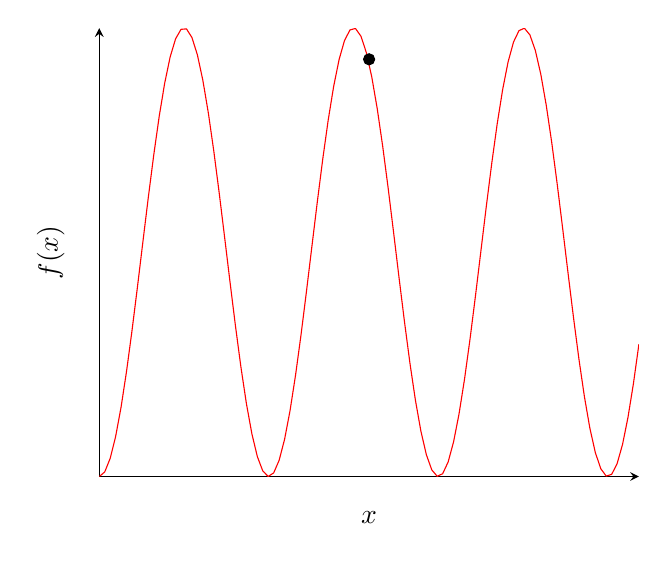
\begin{tikzpicture}
	\begin{axis}[
	    axis lines = left,
	    tick style={draw=none},
	    xticklabels={},
	    yticklabels={},
	    xlabel = $x$,
	    ylabel = {$f(x)$},
	]
	%Below the red parabola is defined
	\addplot [
	    color=red,
	    samples=100,
	]
	{sin(deg(x+5))^2};
    \addplot[mark=*] coordinates {(0,0.93)} node[]{} ;
	\end{axis}
	\end{tikzpicture}  
  \caption{ Non-linear function\\ with a sample point}
  \label{fig:non_lin_function}
\end{minipage}
\end{figure}

Most functions are not constant, however it is possible to turn any function into a constant one. This is exactly what can be done within MC integration. To convert a function $f$ to a constant function, a function $f'$ can be introduced which produces the same output as $f$ for every input, but scaled by a constant $c$ \cite{scratchapixel_2015}. The function $f$ is then divided by $f'$ to produce a constant function, as shown in equation \ref{eq:constant_conversion}.

\begin{equation}
\label{eq:constant_conversion}
\frac{f(x)}{f'(x)} = \frac{1}{c}
\end{equation}

This can be applied to MC integration stated in equation \ref{eq:generalized_mc}, by choosing a PDF  which produces the same output as $f$ for all inputs, but divided by some normalizing constant factor $c$ to ensure the PDF is a probability distribution. Therefore, we are able to calculate the true value of the integral through MC integration as shown in equation \ref{eq:solve_mc_integration}. Where it turns out $\frac{1}{c}$ is the true value for the integral in equation \ref{eq:integral}.

\begin{align}
\label{eq:solve_mc_integration}
\langle F^N \rangle & = \frac{1}{N} \sum^{N-1}_{i=0} \frac{f(x)}{pdf(x)} \\
& = \frac{1}{N} \sum^{N-1}_{i=0} \frac{f(x)}{cf(x)} \nonumber \\
& =  \frac{1}{N} \sum^{N-1}_{i=0} \frac{1}{c} \nonumber \\
& = \frac{1}{c} \nonumber
\end{align}

For most cases, it's not possible to know the correct PDF to sample from which can normalize the function being integrated. However, if one has prior knowledge regarding 'important' regions of the functions input space, it is possible to create a PDF whose shape matches the functions more closely than a uniform PDF. By Important areas of the function input space, we mean areas of the input space which contribute a large amount to the integral of the function.

\begin{figure}[!htb]
\captionsetup{justification=centering}
\centering
\minipage{0.32\textwidth}
\begin{tikzpicture}
	\begin{axis}[every axis plot post/.append style={
	  mark=none,domain=-2:3,samples=50,smooth},
	  axis lines = left,
	  tick style={draw=none},
	  xticklabels={},
	  yticklabels={},
	    % All plots: from -2:2, 50 samples, smooth, no marks
	  axis x line*=bottom, % no box around the plot, only x and y axis
	  axis y line*=left, % the * suppresses the arrow tips
	  enlargelimits=upper,
	  xlabel = $x$,
	  ] % extend the axes a bit to the right and top
	  \addplot [
	  color=red,
	  ]{gauss(0.5,0.8)};
	  \addplot [
	  color=blue,
	  ]{gauss(0.5,1.2)/2};
	\end{axis}
\end{tikzpicture}
  \subcaption{Importance sampling reducing variance}\label{fig:improtance_correct}
\endminipage\hfill
\minipage{0.32\textwidth}
    \begin{tikzpicture}
	\begin{axis}[every axis plot post/.append style={
	  mark=none,domain=-2:3,samples=50,smooth},
	  axis lines = left,
	  tick style={draw=none},
	  xticklabels={},
	  yticklabels={},
	    % All plots: from -2:2, 50 samples, smooth, no marks
	  axis x line*=bottom, % no box around the plot, only x and y axis
	  axis y line*=left, % the * suppresses the arrow tips
	  enlargelimits=upper,
	  xlabel = $x$,
	  ] % extend the axes a bit to the right and top
	  \addplot [
	  color=red,
	  ]{gauss(0.5,0.8)};
	  \addplot [
	  color=blue,
	  ]{0.1};
	\end{axis}
	\end{tikzpicture}  
   \subcaption{Uniform\\ sampling}\label{fig:improtance_uniform}
\endminipage\hfill
\minipage{0.32\textwidth}%
    \begin{tikzpicture}
	\begin{axis}[every axis plot post/.append style={
	  mark=none,domain=-2:3,samples=50,smooth},
	  axis lines = left,
	  tick style={draw=none},
	  xticklabels={},
	  yticklabels={},
	    % All plots: from -2:2, 50 samples, smooth, no marks
	  axis x line*=bottom, % no box around the plot, only x and y axis
	  axis y line*=left, % the * suppresses the arrow tips
	  enlargelimits=upper,
	  xlabel = $x$,
       ] % extend the axes a bit to the right and top
	  \addplot [
	  color=red,
	  ] {gauss(0.5,0.8)};
	  \addplot [
	  color=blue,
	  ]{(-gauss(0.5,1.2) + 0.3)/2};
	\end{axis}
	\end{tikzpicture}  
  \subcaption{Importance sampling increasing variance}\label{fig:improtance_incorrect}
\endminipage
\caption{Graphical representation of a function $f(x)$ (red) and the corresponding PDF $pdf(x)$ (blue) used in the MC integration approximation for the integral of $f(x)$.}
\end{figure}

Figure \ref{fig:improtance_correct} represents a PDF which has a similar shape to the function which is being integrated. Therefore, the variance in the MC integration approximation will be lower then that of the uniform distribution shown in figure \ref{fig:improtance_uniform}. Figure \ref{fig:improtance_incorrect} presents an example where the created probability density function does not resemble the shape of the function which is being integrated. Using this PDF for MC integration would significantly increase the variance in the approximation compared to that from a uniform PDF in figure \ref{fig:improtance_uniform}. This is due to regions which have high importance according to the PDF actually contribute a low amount to the integral of the function $f$, causing the rise in variance of the MC approximation.


\section{Monte Carlo Path Tracing}
\label{sec:mc_pathtracing}
In 1986 James Kajiya introduced the rendering equation and with it, a MC integration approximation to the equation \cite{kajiya1986rendering}. This MC approximation is what is known as today as Monte Carlo path tracing which we refer to as path tracing. Here, we will give a detailed explanation of the rendering equation, what is represents, and how Monte Carlo Path Tracing approximates the equation by light transport simulation. As path tracing involves MC integration, importance sampling can be used to reduce the variance in its approximation, as described in section \ref{sec:importance_sampling}.

\subsection{The Rendering Equation}
\label{sec:rendering_equation}

Equation \ref{eq:rendering_equation} is the rendering equation. It calculates the outgoing radiance from a point $x$ in a direction $\omega$. Radiance indicates the power of light emitted, transmitted, reflected or received by a surface from a given direction. The units of radiance are watts per steradian per square metre $(W \cdot \{sr\}^{-1} \cdot m^{-2})$. Therefore, by placing a camera in a scene, the radiance incident on the lens from a given surface determines the cameras perceived colour and power of light incident from the surface. These values are used to calculate pixel values in computer image generation. The rendering equation states how to correctly perform light transport simulation for rendering, and in turn how to accurately simulate global illumination. Therefore, methods which can accurately approximate the rendering equation for any given scene, are able to convert the incident radiance into pixel values. In turn, with enough SPP these pixel values form a high quality computer graphically generated image. The exact details of this process will be described in section \ref{sec:monte_carlo_path_tracing}.

\begin{equation}
\label{eq:rendering_equation}
\underbrace{L_o(x, \omega)}_{\text{Outgoing}} =\underbrace{ L_e(x,\omega)}_{\text{Emitted}} + \underbrace{\int_\Omega L_i(x, \omega_i)  \cdot f_r(\omega_i, x, \omega) \cdot \cos(\theta_i) d\omega_i}_{\text{Reflected}}
\end{equation}
Where:
\begin{conditions}
 L_o(x, \omega)   &  The total outgoing radiance from a 3D point $x$, in the direction $\omega$  \\
 L_e(x,\omega)     &  The emitted radiance from the point $x$, in the direction $\omega$ \\   
\Omega   &  Hemisphere centred at $x$ oriented to the normal $\mathbf{n}$ of the surface, containing all angles $\omega_i$ \\
L_i(x, \omega_i) & The radiance incident on $x$ in direction $\omega_i$\\
f_r(\omega_i, x, \omega)   & The BRDF, describing the proportion of light reflected from $\omega_i$ in direction $\omega$\\
cos(\theta_i)   &  Cosine of the angle between surface normal at point $x$ and the direction $\omega_i$\\
\end{conditions}

The rendering equation is based on the physical law of the conservation of energy. Where the outgoing radiance in a given direction  from a point ($L_o$), is equal to the emitted light ($L_e$) from that point in that direction, plus the reflected light (the integral) from that point in that direction. The emittance term $L_e$ is simple, it is the light emitted from the point $x$ which has been intersected with. If this is non-zero, a light source has been intersected with. However, the reflected light which is represented by the integral is generally analytically intractable, as it involves summing the contribution of incoming radiance from infinitely many directions in the hemisphere $\Omega$ around the point $x$. Also, the incident radiance function $L_i$ is recursive \cite{dutre2004state}, as to calculate the radiance incident in the direction $\omega_i$ on $x$,  requires a solution to $L_o(h(x, \omega_i), -\omega_i)$. Where $h(x, \omega_i)$ is the hit-point function, which determines the closest intersected position $y \in \mathbb{R}^3$ in the scene by shooting a ray from $x$, in direction $\omega_i$. This concept is represented Figure \ref{fig:recursive_rendering}. Note, the functions $L_o, L_e, L_i$ are all 5-dimensional functions as they both takes a position in the scene $x \in \mathbb{R}^3$ and a direction $\omega \in \mathbb{R}^2$.

\begin{figure}[h]
\begin{center}
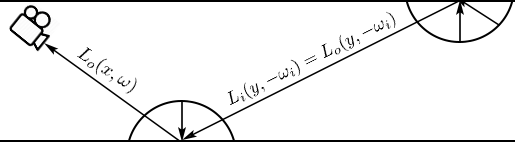
\includegraphics[width=0.7\textwidth]{images/rendering_equation.png}    
\end{center}
\caption{A diagrammatic representation of the recursive nature of the rendering equation. The outgoing radiance ($L_o$) in a given direction $\omega$ from a point $x$ requires an estimation of the incident radiance coming from all angles in the hemisphere around the point, that is $L_i(x,\omega_i)$ $\forall \omega_i \in \Omega$. To calculate $L_i(x, \omega_i)$ is identical to calculating the outgoing radiance $L_o(h(x, \omega_i), -\omega_i)$ as we assume no radiance is lost along a ray line, hence $L_o, L_i$ are recursive functions.}
\label{fig:recursive_rendering}
\end{figure}

The $f_r$ term in Equation \ref{eq:rendering_equation} is known as the bidirectional reflectance distribution function (BRDF). On a high level, the BRDF describes how a surface interacts with light \cite{glassner2014principles}. Every surface has a BRDF which determines the ratio of reflected radiance in direction $\omega$, when a ray intersects with that surface at a given incident direction $\omega_i$. Therefore, querying the BRDF for a surface at point $x$ with an incident ray direction $\omega'$ and given reflected direction $\omega$, that is $f_r(\omega', x , \omega)$,  a single scalar value is returned. Different materials can have vastly different BRDFs. For example, a diffuse material reflects light almost equally in all directions for any angle of incidence, an example of this is paper. Whilst for specular materials, incident rays are reflected in a narrow area around the perfect reflection direction, many metals exhibit specular reflections.  Example BRDFs of both a diffuse and specular surface are depicted in figure \ref{fig:brdfs}.

\begin{figure}[h]
\centering
\minipage{0.32\textwidth}
  
\includegraphics[width=\textwidth]{images/diffuse_brdf.png}   
  \subcaption{Diffuse BRDF}\label{fig:diffuse_brdf}
\endminipage\hspace{5em}
\minipage{0.32\textwidth}
  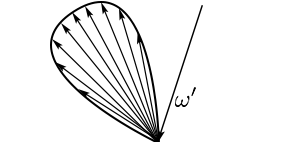
\includegraphics[width=\textwidth]{images/specular_brdf.png}
  \subcaption{Specular BRDF}\label{fig:specular_brdf}
\endminipage
\caption{A representation of both a diffuse surface and specular surface BRDF's for a given angle of incidence $\omega'$. The surface point is located where all outgoing arrows begin. The arrows indicate a subset of directions possible for the incident ray to be reflected in. All possible directions an incident ray be reflected in are defined by any vector which can be formed from the surface point to the curved line for an incident direction $\omega'$. The further away a point is on the curved line, the more likely a ray is to reflected in a direction from the surface point to that point on the curved line. The diffuse surface is equally likely to reflect a ray in any direction. Whereas, the specular surface favours a small subset of directions in the hemisphere surrounding the surface point.}
\label{fig:brdfs}
\end{figure}

Another way to distinguish between diffuse and specular materials is their appearance from different viewing angles. For example, surface of paper appears to be identical no matter the viewing angle. However, a shiny metal ball would appear to reflect what was in front of it, which changes depending on the viewing angle, just like a mirror. These differences can be scene in figure \ref{fig:material_pics}.

\begin{figure}[h]
\centering
\minipage{0.32\textwidth}
  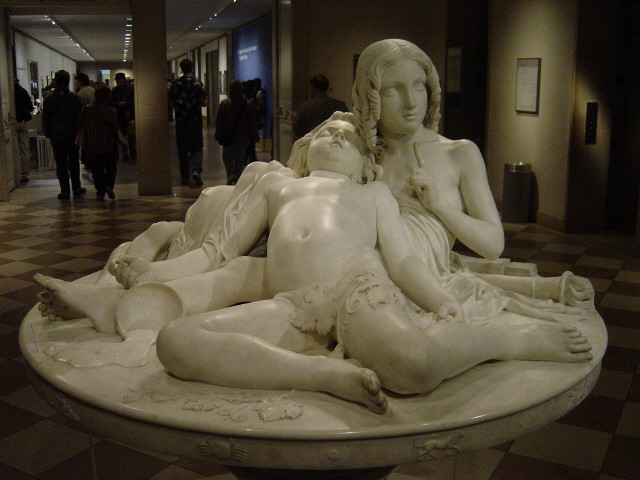
\includegraphics[width=\textwidth]{images/diffuse_sculpture.jpeg}   
  \subcaption{La Table aux Amours, Marble Sculpture}
\endminipage\hspace{5em}
\minipage{0.32\textwidth}
  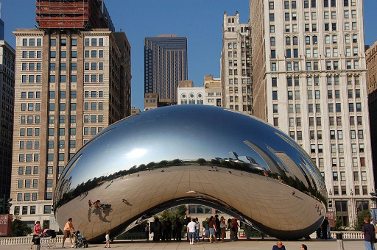
\includegraphics[width=\textwidth]{images/specular_sculpture.jpg}
  \subcaption{Cloud Gate, Stainless Steel Sculpture}
\endminipage
\caption{Two sculptures, one made from a diffuse material (a) and the other from a specular material (b). The specular sculpture appearance is dependent upon the viewing angle, whereas the diffuse sculpture is not.}
\label{fig:material_pics}
\end{figure}

Diffuse materials are generally more computationally expensive to approximate the outgoing radiance $L_o$ from. This is because we have to simulate rays reflecting in all directions around the intersection point on the surface, compared to a specular surface where only a small subset of directions need to be sampled for each intersection. So, from here on whenever a surface or BRDF is mentioned, assume it is diffuse as our descriptions can be extended to specular materials by restricting ray reflections to a limited set of angles.

Finally, as mentioned $\cos(\theta_i)$ is the cosine of the angle between $\omega_i$ and the normal of the intersected surface. The normal of a surface $\mathbf{n}$ is the normalized vector that is perpendicular to the surface \cite{normals}. The $\cos(\theta_i)$ is a weighting for reflected radiance from a point, where the larger the angle from the normal the smaller the reflected radiance. This simulates how light is spread across the surface, causing less light to be reflected in a direction which is further away from being perpendicular to the surface. The combined BRDF and cosine term in the rendering equation uphold the physical law of conservation of energy, meaning more radiance cannot be reflected from the surface then incident on the surface. This is formally described by equation \ref{eq:conservation_energy} \cite{glassner2014principles}, where $\omega_r$ represents a direction of reflection.

\begin{equation}
\forall \omega_i, \int_\Omega f_r(\omega_i, x, \omega_r) \cos(\theta_r) d\omega_r \leq 1
\label{eq:conservation_energy}
\end{equation}

\subsection{Path Tracing}

\subsubsection{Monte Carlo Path Tracing}
\label{sec:monte_carlo_path_tracing}

In section \ref{sec:conceptual_path_trace} we gave a high level overview of the path tracing algorithm. To summarise, many light paths are sampled for each pixel, each sampled light path has a colour estimate. To determine a pixel's colour, the colour estimates for the light paths sampled for the pixel are averaged. It turns out that the process we have just described represents a MC solution to the rendering equation. The proof behind this is detailed in \cite{stanford_graphics}, but conceptually it is simple. 

Previously the reflected radiance for a point $x$ in direction $\omega$ was given by the integral in equation \ref{eq:rendering_equation} with respect to all possible incident angles $\omega_i \in \Omega$ in the hemisphere surrounding $x$. To calculate this integral one can trace infinitely many light paths from the intersection point $x$ in all possible directions $\Omega$ until they intersect with a light source. Each light path approximates the incident radiance in the direction they were sampled. The sum of all these light paths gives the total amount of incident radiance on point $x$. The MC approximation to the rendering equation using the process we have just described is given in equation \ref{eq:rendering_eq_monte_carlo}. Where $L_o^N$ represents the outgoing radiance estimate using $N$ sampled light paths. 

For a given pixel which is intersected with by a direction $\omega$ from point $x$ in the scene, an approximation for $L_o^N(x, \omega)$ directly gives the estimated colour value for that pixel. Therefore, we can render an image by approximating $L_o^N(x, \omega)$ for every pixel in the image.

\begin{equation}
\label{eq:rendering_eq_monte_carlo}
\begin{array}{l}
    L_o^N(x, \omega) = \frac{1}{N} \sum_{k = 0}^{N-1} L_e(x_0, \omega_0) + (L_i(x_0, \omega_1) \cdot f_s(\omega_1, x_0, \omega_0) \cdot cos(\theta_{\omega_1})) / \rho_1\\ 
    \\
   \text{Such that}\\
   \\
    L_i(x_i, -\omega_i) = \begin{cases} 
    L_e(x_i, \omega_i) & \mbox{if } x_i = \mbox{Light Source}\\
    L_e(x_i, \omega_i) + (L_i(x_{i}, \omega_{i+1}) \cdot f_s(\omega_{i+1}, x_{i}, \omega_i) \cdot cos(\theta_{\omega_{i+1}})) / \rho_i & \mbox{otherwise} \end{cases}
\end{array}
\end{equation} 
Where:
\begin{conditions}
 x_i   & Intersection location of the light path after $i$ reflections in the scene\\
 \omega_i   & Direction of the light path after $i$ reflections in the scene\\
 \rho_i   & PDF over reflected ray directions for position $x_i$ evaluated at the angle of incidence $\omega_i$
\end{conditions}

In equation \ref{eq:rendering_eq_monte_carlo} the recursive $L_i$ is still present, but the recursion is terminated when the light path intersects with a light source. By the law of large numbers in equation \ref{eq:law_large_numbers}, the larger the number of sampled light paths (SPP) $N$ for solving equation \ref{eq:rendering_eq_monte_carlo}, the closer the approximated colour value for each pixel will be to its true colour value. Meaning, the more samples used in the Monte Carlo approximation in Equation \ref{eq:rendering_eq_monte_carlo}, the lower the amount of noise in the image \cite{christensen2016path}. To visualise this concept, figure \ref{fig:reduce_noise_spp_example} presents seven rendered images using an increasing number of SPP $N$ for the solution of $L_o^N$. The more samples used, the lower the noise in the rendered image. The pseudo code for a simple path tracer which was used to produce the images in figure \ref{fig:reduce_noise_spp_example} is given in algorithm \ref{alg:forward_path_tracing}.

\begin{figure}[h]
\begin{center}
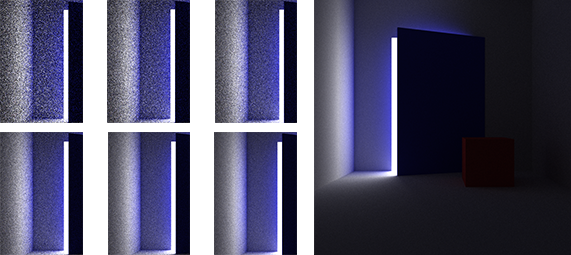
\includegraphics[width=0.99\textwidth]{images/renders/noise_reduction_default/increasing_samples.png}    
\end{center}
\caption{An indirectly illuminated scene produced by path tracing. The grid of image sections show how increasing the number of SPP reduces image noise. Beginning in the top left with 16 SPP, to the bottom right with 512 SPP. The full image on the right is a reference image with 4096 SPP where the MC approximation has almost converged for all pixel values.}
\label{fig:reduce_noise_spp_example}
\end{figure}

\begin{algorithm}[H]
\label{alg:forward_path_tracing}
\SetKwProg{Fn}{Function}{ }{end}
\SetAlgoLined
 \Fn{renderImage(camera, scene)}{  
   \For{$i = 1$ \KwTo $N$}{
     \For{$p$ \In $camera.screen$}{
         \tcc{Set the ray to be traced from the camera, through the pixel and into the scene}
         $ray \leftarrow \text{initializeRay}(p, camera)$\\
         \For{$j=1$ \KwTo $\infty$}{
         \tcc{Find the rays closest intersection with the scene geometry}
         $(y, \mathbf{n}, L_e) \leftarrow \text{closestIntersection}(ray, scene)$\\
         \If{$\text{noIntersection}(y) \ \Or \ \text{areaLightIntersection}(y)$}{
             $ray.throughput \leftarrow ray.throughput \cdot L_e$\\
             $\text{updatePixelColourEstimate}(p, ray.throughput)$\\
             $\Break$
          }
          $(\omega_i, \rho_i, f_s) \leftarrow \text{sampleRayDirRandomly}(y)$\\
          $ray.throughput \leftarrow ray.throughtput \cdot f_s \cdot (\omega_i \cdot \mathbf{n}) / \rho_i$\\
          $ray \leftarrow (y, \omega_i)$
       }
   }
  }
 }
 \caption{Pseudo code for a path tracer. Given a camera position, scene geometry, this algorithm will render a single image by finding the colour estimate for each pixel using Monte Carlo path tracing. Where $N$ is the pre-specified number of sampled light paths per pixel.}
\end{algorithm}


\subsubsection{Importance Sampling in Path Tracing}

As path tracing is a Monte Carlo method for solving the rendering equation, Importance sampling can be applied in order to reduce the variance in pixel colour estimates. In section \ref{sec:importance_smapling}, we showed that by using a PDF which closely matches the shape of the function being integrated, the variance in the Monte Carlo approximation can be significantly reduced. 

The term $\rho_i$ in equation \ref{eq:rendering_eq_monte_carlo} represents the PDF over directions to continue a light path in for intersection location $x_i$, evaluated at direction $\omega_i$. The path tracer in figure \ref{fig:reduce_noise_spp_example} uses a uniform PDF, such that each direction in the hemisphere surrounding an intersection point has a probability of $\rho_i = \frac{1}{2\pi}$ of being sampled. But this can be modified with prior knowledge of which directions are more important for continuing a light path in for a given position in the scene. Important directions are those which leads to a high contribution of radiance incident radiance.

The question now is, do we have any knowlegde of which directions contribute the most radiance for every possible point in the scene? Or in other words, do we have any knowledge of the incident radiance function $L_i(x, \omega)$ for a scene? The answer is yes, and there has been a large amount of research in this topic. The simplest example lies within the rendering equation itself, $cos(\theta_i)$. As previously discussed, this term acts as a weighting for the contribution of radiance from a given direction. So, the probability density function $\rho_i$ can also be weighted by $cos(\theta_i)$, which is likely to reduce the pixel value variance, as our PDF will be closer to the true incident radiance function $L_i$. 

There exists many other methods of retrieving knowledge from the scene to use in importance sampling during rendering. For example, irradiance cahcing \cite{bashford2012significance}, table-driven adaptive importance sampling \cite{cline2008table}, and sequential Monte Carlo adaptation \cite{pegoraro2008towards}. However, these methods suffer from the problem described in \ref{motivation} where they do not account for light blockers. This is because they do not actually attempt to learn a the incident radiance function instead, they make assumptions about its general shape. Meaning if these assumption are incorrect, there is potential that the PDF used by these methods for importance sampling is a far different shape to the true incident radiance function $L_i$. Hence, they may actually increase the presence of noise rendered in images (see section \ref{sec:importance_sampling}) when compared to using a uniform PDF. 

To avoid this issue, NVIDIA proposed that a reinforcement learning method can be adapted and used to learn the incident radiance function. This approximation of the incident radiance function is then used for importance sampling directions to continue light paths in \cite{dahm2017learning}, leading to a reduction in image noise. We will present NVIDIA's path tracer in chapter \ref{chap:td_deep_sampling}


\section{Reinforcement Learning and TD-Learning}

In this section we give a quick introduction to reinforcement learning and TD-learning. TD-learning learning rules are what both we and NVIDIA propose to use for approximating the incident radiance function. This approximation is used to importance sample directions to continue light paths in, in order to reduce the noise present in images rendered by path tracing. Exactly how the TD-learning can be applied to learn the incident radiance function is the central topic of chapter \ref{chap:td_deep_sampling}.

\subsection{Markov Decision Processes}
Reinforcement learning is one of the three archetypes of machine learning. It is concerned with finding what action should be taken in a given situation, in order to maximise a numerical reward \cite{sutton2011reinforcement}. This problem is formalized by a finite Markov Decision Process (MDP), which is designed to capture the most important aspects of the problem a learning agent faces when interacting over time with its environment to achieve a goal. An MDP is summarised in figure \ref{fig:mdp} and can be described in terms of the following:

\begin{itemize}
\item \textbf{Agent} - The learner and decision maker which takes an action $A_t$ in an observed state $S_t$ (where $t$ is the current time step), receiving an immediate numerical reward $R_{t_+1}$ and the next observed state $S_{t+1}$

\item \textbf{Environment} - What the agent interacts with when taking an action $A_t$ in state $S_t$ and produces both $R_{t+1}$ \& $S_{t+1}$ 
\end{itemize}

\begin{figure}[h!]
\begin{center}
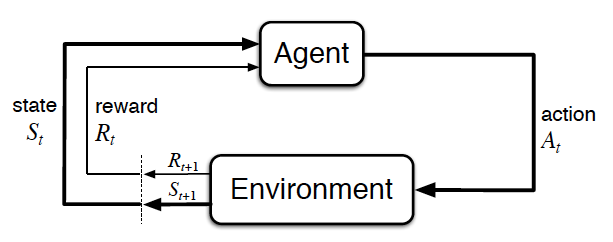
\includegraphics[width=0.5\textwidth]{images/MDP.png}    
\end{center}
\caption{Markov Decision Process \cite{sutton2011reinforcement}}
\label{fig:mdp}
\end{figure}

\noindent
An MDP comprises of the following the following tuple:

$$(\mathcal{S}, \mathcal{A}, p,\gamma)$$
Where:
\begin{conditions}
\mathcal{S}   &  The set of all states\\
\mathcal{A}   &  The set of all actions\\
p   & Probability of receiving reward $r$ and state $s'$ when in the previous state $s$ and action $a$ was taken\\
\gamma   & The discount factor which makes the agent value immediate rewards higher than later ones \\
\end{conditions}

\noindent
An important detail of an MDP  is that any problem modelled by an MDP assumes the Markov property.

\begin{quote}
"The future is independent of the past, given the present." - \textit{Hado van Hasselt, Senior Research Scientist at DeepMind} \cite{introToRL}
\end{quote}

This is expressed mathematically for an MDP in equation \ref{eq:markov_property}. Put simply, the Markov property means the current state captures all relevant information from the history of all previous states the agent has experienced. Meaning the history of all previous states are not needed if we have the current state.

\begin{equation}
\label{eq:markov_property}
p(R_{t+1} = r, S_{t+1} = s' | S_t = s) = p(R_{t+1} = r, S_{t+1} = s' | S_1, .. , S_{t-1}, S_{t})
\end{equation}

\subsection{Goals and Rewards}
The goal of a reinforcement learning agent can change significantly depending on the problem. For example, in the case of a game it may be to maximise the total score in one play-through. Or for a robotic space rover, it may be to discover the most amount of unseen terrain. However, in terms of an MDP all AI agents goals are described as maximising the total amount of cumulative reward received. This is more formally described by the reward hypothesis \cite{sutton2011reinforcement}:

\begin{quote}
Any goal can be formalized as the maximisation of the expected value of the cumulative sum of a received scalar reward signal.
\end{quote}

Once again, in the case of an agent learning the best possible action to take for any state in a game, a reward signal could be the points gained by making a certain move. Therefore, to maximise the expected return would be to maximise the number of points received in a play-through of the game in this case.  The return is formally defined in equation \ref{eq:return}. It consists of a sequence of reward signals ($R_{t+i}$), combined with the discount factor ($\gamma$), which as previously mentioned trades off later rewards for more immediate ones. If the discount factor is closer to 1, the agent is said to be far sightes, as it gives future rewards a high weighting. Whereas a myopic agent is one which has a discount factor closer closer to 0, as it gives a lower weighting to future rewards for their contribution towards the return $G_t$ \cite{introToRL}. 

\begin{equation}
\label{eq:return}
G_t = R_{t+1} + \gamma R_{t+2} + \gamma^2 R_{t+3} + ... = \sum^\infty_{k=0} \gamma^k R_{t+k+1}
\end{equation}

This formulation works well if the agents interactions with the environment break down easily into sub-sequences \cite{sutton2011reinforcement}. Where an agent starts in one of a given set of \textit{starting states} and takes a series of actions to reach a \textit{terminal state}. The process of taking a series of actions from the starting state to the terminal state is known as an \textit{episode}. From the terminal state the agent can be reset to one of the starting states to begin learning once again. This applies to path tracing, where the terminal state is one in which the light path has intersected with a light. This will be discussed in detail in chapter \ref{chap:td_deep_sampling}.

\subsection{Value Function and Optimality}
\label{sec:optimal_value}
All reinforcement learning algorithms we will be considering involve the concept of a value function. There are two kinds of value functions, one which determines the value of being in a given state, the other determines the value of being in a certain state and taking a certain action, known as a state-action pair. We will be focusing on state-action pair value functions, where the value of a state-action pair is defined in terms of the expected return $G_t$ from that state-action pair.

An agent follows a policy $\pi$, which determines how the agent will act in a given state. More formally, a policy is a mapping from states to probabilities of selecting a particular action. When an agent is following policy $\pi$ at time $t$, then $\pi(a|s)$ is the probability of the agent taking action $A_t = a$ in state  $S_t = s$. The reinforcement learning algorithms we shall discuss state how an agents policy changes from experience. In other words, how the agents behaviour changes depending on previous experiences.

The value of a state-action pair $(s,a)$ under a policy $\pi$, is given in equation \ref{eq:value_function} denoted as $q_\pi(s,a)$,. This value function is commonly known as the action value function for policy $\pi$. Stating 'under policy $\pi$' is important as the value of a given state-action pair depends upon the actions we take onwards from taking action $a$ in state $s$ while following $\pi$. $\mathbf{E}_\pi$ denotes the expected value of a random variable, given that the agent follows policy $\pi$. From this, if we were to keep track of the actual returns received for taking a state-action pair, then as the number of times all state-action pairs are chosen tends to infinity, the average of the returns for the state action pair $(s,a)$ will converge on the true expected value of the return for that state-action pair $q_\pi(s,a)$.

\begin{equation}
\label{eq:value_function}
q_\pi(s, a) = \mathbf{E}_\pi[G_t | S_t = s, A_t = a] = \mathbf{E}_\pi [\sum_{k=0}^{\infty} \gamma^k R_{t+k+1} | S_t = s, A_t = a]
\end{equation}

Now, if we had an AI agent the best way it could perform would be to maximise the true expected reward it receives in an episode. The policy which does this is known as the \textit{optimal policy}, which is provably better than all other policies an agent can follow. Formally, the optimal policy is $\pi$ if $\pi \geq \pi'$ for al possible policies $\pi'$. Where, $\pi \geq \pi'$ if and only if $q_\pi(s,a) \geq q_{\pi'}(s,a)$ for all $s \in \mathcal{S}$ and $a \in \mathcal{A}$. The optimal policy is denoted as $\pi_*$ and the value function following the optimal policy, which is the \textit{optimal value function}, is denoted $q_*(s,a)$. The optimal value function is defined in equation \ref{eq:optimal_value}.

\begin{align}
q_*(s,a) & = \max_\pi q_\pi(s,a) \label{eq:optimal_value} \\
 & = \mathbf{E}[R_{t+1} + \gamma \max_{a'} q_* (S_{t+1}, a') | S_t = s, A_t = a]  \label{eq:bellman_optimal}
\end{align}

Equation \ref{eq:bellman_optimal} defines the \textit{Bellman optimality equation}, which states that the value of a state-action pair under an optimal policy must be equal to the expected return of the immediate reward plus the highest valued state-action pair available from the next state. Intuitively, if the optimal policy is available which is essentially a cheat sheet of what action is most valuable to take in each state. Then the trhe value of a given state-action pair should be equal the immediate reward received by taking the action in the current state, plus the value of the best action to take in the next state given by the cheat sheet/optimal policy. SImilarly, if we have the optimal value function, the optimal policy can easily be found by choosing the action $a$ with the highest values $q_*(s,a)$  in state $s$ \cite{sutton2011reinforcement}. 

To summarize, the aim from here on is to build an agent which is able to learn the optimal value function. But whilst this is provably possible, it rarely happens in practice. However, the learning methods I will discuss in the next section on TD-learning are able to learn a good value function in practice \cite{sutton1996generalization, konidaris2011value, uther1998tree, mnih2013playing}.

\subsection{Temporal Difference Learning}
\label{sec:td_learning}

TD-Learning is combination of Monte Carlo and Dynamic Programming reinforcement learning methods for learning the optimal value function from equation \ref{eq:optimal_value}. We will not discuss the details of Monte Carlo and Dynamic Programming methods as they are not investigated as part of our work. However, the reasoning for choosing to study  TD-learning approaches over these two alternative approaches are as follows; TD-learning can perform learning updates of the value function throughout an episode, unlike Monte Carlo approaches which wait until the end \cite{model_free_prediction}. This means TD-learning algorithms can be implemented as online learning algorithm \cite{sutton2011reinforcement}, meaning they are able to learn during an episode. TD-learning can learn directly from experience, as it does not require a true model of the environment in order to learn the optimal value function, unlike Dynamic Programming methods \cite{mdp_dynamic_prog}. This means TD-learning is model-free, avoiding the expense of building the true model of the environment.

We will now introduce three different TD-learning methods which are required knowledge for the rest of our work.

\subsubsection*{Sarsa}

Sarsa is an on-policy TD method which learns a state-action pair valuation function $q_\pi(s,a)$. The Sarsa learning rule is presented in equation \ref{eq:sarsa}, and we have chosen to present this method first to explain some key concepts TD-learning methods share. Firstly, $Q$ denotes the current apporximation of the optimal value function under policy $\pi$, $q_\pi$. Therefore the left arrow indicates an update in the currently estimated value of state-action pair $(s,a)$, $Q(s,a)$. Also notice, how the current estimate is update upon every time step $t$, this means Sarsa like other TD-learning methods can learn during an episode as previously mentioned. The $\alpha$ term is the current learning rate, where $\alpha \in [0,1]$ and $\gamma$ is the discount factor as previously described. Finally, Sarsa performs what is known as bootstrapping in the context of reinforcement learning \cite{sutton2011reinforcement}. Bootstrapping is where the current estimate of the value function ($Q$) is updated based on some new data received by experience, which is the immediate reward $R_{t+1}$. As well as, the current estimate of the value function $Q$. Sarsa therefore learns from experience after every time step $t$, whereby an action $A_t$ is taken in state $S_{t}$, leading to an immediate reward $R_{t+1}$ which is used to update the current estimate $Q$.

\begin{equation}
Q(S_t, A_t) \leftarrow Q(S_t, A_t) + \alpha[R_{t+1} + \gamma Q(S_{t+1}, A_{t+1}) - Q(S_t, A_t)]
\label{eq:sarsa}
\end{equation}

The reasoning behind the name Sarsa is that the method uses every element in the quintuple, $(S_t, A_t, R_{t+1}, S_{t+1}, A_{t_1})$, which makes up a transition between each time step of state-action pairs. Sarsa is an on-policy TD-learning method, as to choose the next action to take in the next state ($Q(S_{t+1}, A_{t+1}$) the policy is used. Sarsa is proven to converge on the optimal value function $q_*$ when the policy $\pi$ remains constant. Sarsa is a tabular learning method for approximating the optimal value function $q_*$. Meaning, a table with an entry for every state-action pair is required for the algorithm to converge on the optimal value function by using the update rule in equation \ref{eq:sarsa}.

To make Sarsa learning and TD-learning in general more concrete, imagine a robot with a camera whose goal it is to manoeuvre to the end of a corridor. Each time step is the point when a new frame is rendered on the camera, and the state is the image displayed by the camera. The robots actions consist of moving a short distance in a set of four different directions. If the robot were to learn using Sarsa, the robot would have a large table storing the value of each state-action pair $Q(S_t, A_t)$, which represents the current approximation of the value function. The robot would then select an action at each time step according to the policy $\pi$ to receive a reward signal based on its distance to the end of the corridor. The robot would then perform a lookup on the large table, indexing with the action it took in the state it was in to perform the update rule in \ref{eq:sarsa}. This large table representing the current estimate of the optimal value function is also know as a \textit{Q-table}, where each value in the table is known as a \textit{Q-value}, $Q(S_t, A_t)$. By following a suitable policy, the robot will over time will keep updating its Q-values to improve
its estimate of $q_\pi(s,a)$.

\subsubsection{Q-Learning}

Q-learning is very similar to Sarsa except it is an off-policy TD-learning algorithm. Also, if all state-action pairs are visited infinitely many times, it is proven that Q-learning can converge on the optimal policy $q_\pi(s,a)$ faster than Sarsa. Making it a generally a preferred method to Sarsa. The learning rule is given in equation \ref{eq:q_learning}, where rather than following a policy $\pi$ to select the action to update with, the maximum value of the highest valued action in the next state is selected ($\max_a Q(S_{t+1}, a$). This means the agent following policy $\pi$ will still choose its actions from a state based on $\pi$, however when it updates its value function $Q$, the action it chooses to update with may not necessarily be the same as the action it took. Hence, Q-learning is an off-policy TD-learning algorithm.

\begin{equation}
Q(S_t, A_t) \leftarrow Q(S_t, A_t) + \alpha[R_{t+1} + \gamma \max_aQ(S_{t+1}, a) - Q(S_t, A_t)]
\end{equation}

\subsubsection{Expected Sarsa}

Expected Sarsa is a TD-learning algorithm which is generally found to be superior to both Q-learning and Sarsa in practice \cite{sutton2011reinforcement}. It is very similar to Q-learning, but instead of using the maximum value of the next state-action pairs, it uses the expectation over them. This means Expected Sarsa takes into account how likely each action is under the current policy as shown in equation \ref{eq:expected_sarsa}. Where $\pi(a | S_{t+1})$ returns the probability of selecting action $a$ in state $S_{t+1}$, while following the policy $\pi$. Note, Expected Sarsa may be used as either an on-policy or an off-policy algorithm. For example, if the policy $\pi$ was set to the greedy-policy used in Q-learning, the learning rule would become identical to that of Q-learning. Therefore, Expected Sarsa generalizes over Q-learning. Expected Sarsa also reduces the variance in the value function approximation compared to that of Sarsa, as the expectation taken over the current valuation estimate for state-action pairs used.

\begin{align}
Q(S_t, A_t) &  \leftarrow Q(S_t, A_t) + \alpha [R_{t+1} + \gamma \mathbf{E}[Q(S_{t+1}, A_{t+1}) | S_{t+1}] - Q(S_t, A_t)] \nonumber \\
 & \leftarrow Q(S_t, A_t) + \alpha [R_{t+1} + \gamma \sum_a \pi(a| S_{t+1}) Q(S_{t+1}, a) - Q(S_t, A_t)]
 \label{eq:expected_sarsa}
\end{align}

\subsection{Exploration vs Exploitation}
\label{sec:exploration_vs_exploitation}

Up to now we have formally introduced what reinforcement learning is, including what the optimal value function is and different ways to learn it. In the case of off-policy methods like Q-learning, we have not yet discussed any details about the kind of policy an agent should use to select actions for learning the optimal value function. Deciding on this policy is very influential on our agents performance, as the agent needs to gather enough information about its environment to make the best overall decisions. Therefore, online decision-making requires a fundamental choice to be made by the agent every time it chooses to take an action \cite{exploration_vs_exploitation}. This is between the following:

\begin{itemize}
\item \textbf{Exploration}: Maximise the agents performance based on the current knowledge available
\item \textbf{Exploration}: Gain more knowledge about the environment
\end{itemize}

This means a good learning strategy for an agent may be to sacrifice short-term performance to maximise it in the long-term. This applies directly to the policies used for both on-policy and off-policy TD-learning methods. Initially exploration is the most important to quickly gain a broad amount of knowledge about the environment to open up more specific areas for further exploration. Then over time the policy should favour exploitation more and more by taking known higher valued actions. An example of this kind of policy is the decaying $\epsilon$-greedy policy \cite{sutton2011reinforcement}. This policy maintains the current value of $\epsilon \in [0,1]$ and involves sampling a random number $x \in [0,1]$, then if $x > \epsilon$ exploitation occurs, else exploration. By exploitation it could be to choose the current highest valued action from a state, whereas exploration involves choosing one at random. Overtime $\epsilon$ is decayed by a value $\delta$ as more episodes of training are accumulated, achieving the behaviour of increasing exploitation as more knowledge is gained.

\section*{Summary}
The story up to this point can be summarised as follows; Monte Carlo integration is a numerical technique for approximating integral. It can be used to find an approximation of pixel values in path tracing by approximating the reflected radiance from a point in a given direction. Rather then uniformly sampling directions in light path construction for determining pixel values, a whole field is dedicated to importance sample these directions to reduce the variance in the Monte Carlo approximation. However, most traditional methods do not learn the incident radiance function, limiting their effectiveness for reducing image noise. Instead, reinforcement learning, specifically temporal difference learning techniques can be applied to learning the outgoing radiance from a point in a given direction, which are in turn used for importance sampling ray directions where the approximated radiance is high. We are specifically interested in TD-learning methods which are used to approximate the optimal value function, which in turn is used to make a better decision on what action an agent should take from a given state.

\begin{comment}
{\bf A compulsory chapter,     of roughly $10$ pages} 
\vspace{1cm} 

\noindent
This chapter is intended to describe the technical basis on which execution
of the project depends.  The goal is to provide a detailed explanation of
the specific problem at hand, and existing work that is relevant (e.g., an
existing algorithm that you use, alternative solutions proposed, supporting
technologies).  

Per the same advice in the handbook, note there is a subtly difference from
this and a full-blown literature review (or survey).  The latter might try
to capture and organise (e.g., categorise somehow) {\em all} related work,
potentially offering meta-analysis, whereas here the goal is simple to
ensure the dissertation is self-contained.  Put another way, after reading 
this chapter a non-expert reader should have obtained enough background to 
understand what {\em you} have done (by reading subsequent sections), then 
accurately assess your work.  You might view an additional goal as giving 
the reader confidence that you are able to absorb, understand and clearly 
communicate highly technical material.
\end{comment}

\end{document}